\documentclass[9pt, aspectratio=169]{beamer}

\usetheme{metropolis}
\setbeamertemplate{itemize items}{\faAngleRight}

\metroset{titleformat=smallcaps,block=fill,numbering=counter,progressbar=frametitle,sectionpage=none}
\setbeamersize{text margin left=5mm,text margin right=5mm} 
% %%%%%%%%%%%%%%%%%%%%%%%%%%%%%%%%%%%%%%%%%%%%%%%%%%%%%%%%%%%%%%%%%%%%%%%%%%%%%%
% \embedvideo{<poster or text>}{<video file (MP4+H264)>}
% \embedvideo*{...}{...}                     % auto-play
%%%%%%%%%%%%%%%%%%%%%%%%%%%%%%%%%%%%%%%%%%%%%%%%%%%%%%%%%%%%%%%%%%%%%%%%%%%%%%

\usepackage[bigfiles]{pdfbase}
\ExplSyntaxOn
\NewDocumentCommand\embedvideo{smm}{
  \group_begin:
  \leavevmode
  \tl_if_exist:cTF{file_\file_mdfive_hash:n{#3}}{
    \tl_set_eq:Nc\video{file_\file_mdfive_hash:n{#3}}
  }{
    \IfFileExists{#3}{}{\GenericError{}{File~`#3'~not~found}{}{}}
    \pbs_pdfobj:nnn{}{fstream}{{}{#3}}
    \pbs_pdfobj:nnn{}{dict}{
      /Type/Filespec/F~(#3)/UF~(#3)
      /EF~<</F~\pbs_pdflastobj:>>
    }
    \tl_set:Nx\video{\pbs_pdflastobj:}
    \tl_gset_eq:cN{file_\file_mdfive_hash:n{#3}}\video
  }
  %
  \pbs_pdfobj:nnn{}{dict}{
    /Type/RichMediaInstance/Subtype/Video
    /Asset~\video
    /Params~<</FlashVars (
      source=#3&
      skin=SkinOverAllNoFullNoCaption.swf&
      skinAutoHide=true&
      skinBackgroundColor=0x5F5F5F&
      skinBackgroundAlpha=0
    )>>
  }
  %
  \pbs_pdfobj:nnn{}{dict}{
    /Type/RichMediaConfiguration/Subtype/Video
    /Instances~[\pbs_pdflastobj:]
  }
  %
  \pbs_pdfobj:nnn{}{dict}{
    /Type/RichMediaContent
    /Assets~<<
      /Names~[(#3)~\video]
    >>
    /Configurations~[\pbs_pdflastobj:]
  }
  \tl_set:Nx\rmcontent{\pbs_pdflastobj:}
  %
  \pbs_pdfobj:nnn{}{dict}{
    /Activation~<<
      /Condition/\IfBooleanTF{#1}{PV}{XA}
      /Presentation~<</Style/Embedded>>
    >>
    /Deactivation~<</Condition/PI>>
  }
  %
  \hbox_set:Nn\l_tmpa_box{#2}
  \tl_set:Nx\l_box_wd_tl{\dim_use:N\box_wd:N\l_tmpa_box}
  \tl_set:Nx\l_box_ht_tl{\dim_use:N\box_ht:N\l_tmpa_box}
  \tl_set:Nx\l_box_dp_tl{\dim_use:N\box_dp:N\l_tmpa_box}
  \pbs_pdfxform:nnnnn{1}{1}{}{}{\l_tmpa_box}
  %
  \pbs_pdfannot:nnnn{\l_box_wd_tl}{\l_box_ht_tl}{\l_box_dp_tl}{
    /Subtype/RichMedia
    /BS~<</W~0/S/S>>
    /Contents~(embedded~video~file:#3)
    /NM~(rma:#3)
    /AP~<</N~\pbs_pdflastxform:>>
    /RichMediaSettings~\pbs_pdflastobj:
    /RichMediaContent~\rmcontent
  }
  \phantom{#2}
  \group_end:
}
\ExplSyntaxOff
%%%%%%%%%%%%%%%%%%%%%%%%%%%%%%%%%%%%%%%%%%%%%%%%%%%%%%%%%%%%%%%%%%%%%%%%%%%%%%

\usepackage{fontspec,minted}
\usepackage[scale=1]{ccicons}
\usepackage{metalogo}
\usepackage{xcolor,colortbl}
\usepackage{multicol,multirow,booktabs}
\usepackage{appendixnumberbeamer}
\usepackage{graphicx}
\usepackage{bm}
\usepackage{fontawesome}
\usepackage{csquotes}
\usepackage[backend=biber, natbib, sorting=nyt, doi=true, url=false, url=false, isbn=false, maxbibnames=10]{biblatex}
\addbibresource{../../utils/refs.bib}

\usepackage[spanish]{babel}
\usepackage{mathtools}
\usefonttheme{professionalfonts}
\usepackage{textcomp}

\setsansfont[BoldFont={Iwona Bold}, Numbers={Lining, Proportional}]{Iwona Light}
% \setmathsfont(Digits)[Numbers={Lining, Proportional}]{Fira Sans Light}
\setmonofont[Scale=MatchLowercase]{DejaVu Sans Mono}

\setbeamercolor{alerted text}{fg=red,bg=black!2}
\setbeamercolor{progress bar}{fg=red,bg=red!2}
\setbeamertemplate{itemize item}{\faCaretRight}
\setbeamertemplate{itemize subitem}{ \faAngleRight}
\setbeamertemplate{blocks}[shadow=false]
\setbeamercolor{block title}{bg=black!30,fg=red}
\setbeamercolor{block body}{bg=black!20,fg=black}
 
\usepackage{gensymb,amssymb}
\usepackage{upquote}
\usepackage{algpseudocode}
\algrenewcommand\algorithmicrequire{\textbf{Requiere}}
\algrenewcommand\algorithmicensure{\textbf{Devuelve}}
%\setbeamertemplate{blocks}[rounded][shadow=false]
\setbeamertemplate{blocks}[shadow=false]

\newcommand{\cx}{\column{0.5\textwidth}}
\newcommand{\cw}[1]{\column{#1\textwidth}}

\author{Manuel Carlevaro}
\date{{\tiny Departamento de Ingeniería Mecánica \\[-1em]
             Grupo de Materiales Granulares - UTN FRLP \\
        \faEnvelope{} manuel.carlevaro@gmail.com \- $\cdot$ \- \faTwitter{} @mcarlevaro}}
\institute{
  \vspace{6em}
  \centering
  {\tiny
  Cálculo Avanzado \enspace • \enspace 2022 \\
    \faLinux \- $\cdot$ \- \fontspec{TeX Gyre Pagella}\XeLaTeX \- $\cdot$ \- \ccbysa }
}

%% Operadores
\DeclareMathOperator{\sen}{sen}
\DeclareMathOperator{\sign}{sign}
\newcommand{\T}[1]{\underline{\bm{#1}}}
\DeclareMathOperator{\Tr}{Tr}

\usepackage{hyperref}
\hypersetup{
    colorlinks,
    citecolor=blue,
    filecolor=black,
    linkcolor=blue,
    urlcolor=blue
}
\urlstyle{same}

%% Códigos
\usepackage{minted}
\newminted[cpp]{cpp}{linenos,fontsize=\footnotesize,frame=lines,numbersep=4pt}
\newmintedfile[cppcode]{cpp}{linenos,fontsize=\footnotesize,frame=lines,numbersep=4pt}
\newcommand{\mic}[1]{\mintinline{C++}{#1}}

\newminted[py]{python}{linenos,fontsize=\footnotesize,frame=lines,numbersep=4pt}
\newminted[pyc]{pycon}{linenos,fontsize=\footnotesize,frame=lines,numbersep=4pt} % Consola de Python
\newminted[ipy3]{ipython3}{linenos,fontsize=\footnotesize,frame=lines,numbersep=4pt} % Consola de iPython3
\newmintedfile[pycode]{python}{linenos,fontsize=\footnotesize,frame=lines,numbersep=4pt}

\newmintedfile[makef]{basemake}{linenos,fontsize=\footnotesize,frame=lines,numbersep=4pt}
\definecolor{bg}{RGB}{22,43,58}
\newminted[shell]{console}{linenos=false,fontsize=\footnotesize,breaklines=true, frame=single} % Linea de comandos
\renewcommand\listingscaption{Código}

\makeatletter
\AtBeginEnvironment{minted}{\dontdofcolorbox}
\def\dontdofcolorbox{\renewcommand\fcolorbox[4][]{##4}}
\makeatother

% uso:
% Ejemplo de uso explícito:
% \begin{py}
% >>> list("abcd")
% ['a', 'b', 'c', 'd']
% \end{py}
% 
% Ahora ejemplo de código en file:
% \pycode{Chapters/intro/code/hola.py}
% 
% También se puede poner un sector del file:
% \pycode[firstline=6, lastline=7]{Chapters/intro/code/hola.py}
% 
% También se puede poner código \textit{inline}: \mip{print('¡Hola mundo!')} y en una sola línea:
% \slp|if __name__ == '__main__')|
% 
% Por último, se puede poner el código en un entorno \textit{float}, esto es, como las tablas y las figuras, con un caption y un label para luego hacer referencias, como por ejemplo al Código \ref{code:hola}.


\usepackage{tikz}
\usetikzlibrary{shapes,shadows,arrows,positioning,matrix,chains,backgrounds,fit}

\tikzset{
    %Define standard arrow tip
    >=stealth',
    %Define style for boxes
    obj/.style={
           rectangle,
           rounded corners,
           draw, very thick,
           text width=10em, fill=green!20,
           minimum height=2em,
           text centered, drop shadow},
    proc/.style={
	    rectangle, rounded corners,
	    draw,fill=red!50,very thick,
	    text width=8em,minimum height=2em,
	    text centered, drop shadow},
    % Define arrow style
    pil/.style={
           ->,
           thick,
           shorten <=2pt,
           shorten >=2pt,}
}

\setbeamertemplate{bibliography item}{%
  \ifboolexpr{ test {\ifentrytype{book}} or test {\ifentrytype{mvbook}}
    or test {\ifentrytype{collection}} or test {\ifentrytype{mvcollection}}
    or test {\ifentrytype{reference}} or test {\ifentrytype{mvreference}} }
    {\setbeamertemplate{bibliography item}{\faBook}}
    {\ifentrytype{online}
            {\setbeamertemplate{bibliography item}{\faGlobe}}
   {\setbeamertemplate{bibliography item}{\faFileText}}}%
  \usebeamertemplate{bibliography item}}

\defbibenvironment{bibliography}
  {\list{}
     {\settowidth{\labelwidth}{\usebeamertemplate{bibliography item}}%
      \setlength{\leftmargin}{\labelwidth}%
      \setlength{\labelsep}{\biblabelsep}%
      \addtolength{\leftmargin}{\labelsep}%
      \setlength{\itemsep}{\bibitemsep}%
      \setlength{\parsep}{\bibparsep}}}
  {\endlist}
  {\item}
\newcommand{\bcite}[1]{\citeauthor{#1}, \citetitle{#1} (\citeyear{#1})}


\title{Introducción a la variable compleja}
\subtitle{Introducción al curso.\\ Números complejos (repaso). Funciones de variable compleja. Límite y continuidad. Diferenciabilidad y funciones analíticas.}


\begin{document}
\maketitle

\begin{frame}{ Presentación }
    \begin{columns}[t]
    \cx
    \textbf{Docentes:}
    \begin{itemize}
    \item Profesor: Manuel Carlevaro
    \item Jefe de Trabajos Prácticos: Diego Amiconi
    \item Ayudante de Primera: Lucas Basiuk
    \end{itemize}
    \vspace{1em}

    \textbf{Clases:}
    \begin{itemize}
    \item Miércoles de 18:15 a 20:30
    \item Teoría + práctica
    \item Clases de consulta: horario a confirmar
    \end{itemize}
    \cx
    \textbf{Evaluación:}
    \begin{itemize}
    \item Trabajos prácticos (8)
    \item Parciales 2 (+ 2 recuperatorios)
    \item Aprobación directa: TPs + 2 parciales ($\geq 6$)
    \item Aprobación no directa - examen final: al menos un parcial con 4 o 5 
    \end{itemize}
    \end{columns}
\end{frame}

\begin{frame}{Programa}
\begin{columns}[t]
\cx 
\begin{enumerate}
    \item Introducción a la variable compleja (2 clases)
    \item Transformada y serie de Fourier (2 clases - TP1)
    \item Transformada de Laplace (1 clase - TP2)
    \item Errores en el cálculo numérico (1 clase)
    \item Cálculo de raíces: soluciones de una variable (2 clases - TP3)
    \item Normas de vectores y matrices (2 clases)
    \item Autovalores y autovectores (2 clases - TP4)
\end{enumerate}
\cx 
\begin{enumerate}
    \setcounter{enumi}{7}
    \item Resolución de sistemas de ecuaciones lineales (2 clases - TP5)
    \item Aproximación discreta y continua por el método de los mínimos cuadrados (dos clases - TP6)
    \item Resolución de problemas de valor inicial (dos clases - TP7)
    \item Resolución de problemas de contorno (dos clases)
    \item Resolución de ecuaciones diferenciales de segundo orden mediante diferencias finitas (2 clases - TP8)
\end{enumerate}
\end{columns}
\vspace{1em}
\begin{columns}[c]
\cx
\centering
\only<1>{\phantom{\alert{Primer parcial: 12/07} }}
\only<2>{\alert{Primer parcial: 12/07} }

\cx
\centering
\only<1>{\phantom{\alert{Segundo parcial: 22/11} }}
\only<2>{\alert{Segundo parcial: 22/11} }
\end{columns}
\end{frame}

\begin{frame}{Recursos}
\textbf{Específicos de Cálculo Avanzado:}
\begin{itemize}
    \item CVG: \href{https://frlp.cvg.utn.edu.ar/course/view.php?id=189}{Cálculo Avanzado}
    \item GitHub: \url{https://github.com/manuxch/calculo_avanzado}
\end{itemize}

\textbf{Recursos adicionales:}
\begin{itemize}
    \item Python y programación: \url{https://github.com/gmg-utn/compTools}
    \item \LaTeX - \XeLaTeX: \url{https://es.wikibooks.org/wiki/Manual_de_LaTeX}
\end{itemize}
\end{frame}

\begin{frame}{Bibliografía}
    \begin{columns}[t]
    \cw{0.45}
    \begin{itemize}
    { \small 
    \item \fullcite{kreyszig2011}.
    \item \fullcite{spiegel2011}.
    \item \fullcite{brown2004}.
    \item \fullcite{oneil2012}.
    \item \fullcite{edwards2009}.
    \item \fullcite{burden2017}.
    }
    \end{itemize}

    \cw{0.45}
    \begin{itemize}
    { \small 
            \item \fullcite{nr2007}.
            \item \fullcite{gupta2019}.
            \item \fullcite{strang2006}.
            \item \fullcite{pine2019}.
            \item \fullcite{langtangenLinge2016}.
            \item \fullcite{batista2023}.
    }
    \end{itemize}
    \end{columns}
\end{frame}

\begin{frame}[standout]
    \centering
    ¿Preguntas, dudas, comentarios?
\end{frame}

\begin{frame}{Los números complejos}
 \begin{columns}[t]
  \cw{0.3}
  Sistema de enteros:
  \begin{align*}
  2 x &= 3 \\
  x &= \;?
  \end{align*}
  
  Números ``reales'': $\{ x: x^2 \geq 0\}$
  \begin{align*}
   x^2 &= -1 \\
   x &= \;?
  \end{align*}
  
  Motivación: $ x^2 + 1 = 0 $ ¿tiene solución?
  
  Ejemplo: usar $y = e^{rx}$ para resolver:
  \[  y'' + y = 0 \]
  
  \cw{0.3}
  \begin{align*}
   & r^2 e^{rx} + e^{rx} = 0 \\
   & \therefore r^2 + 1 = 0 \therefore r = \pm \sqrt{-1} = \pm i \\
   & \therefore y = e^{ix} \text{ o } y = e^{-ix} \\
   & \boxed{y = \cos x \text{ o } y = \sen x}
  \end{align*}
  
  De ``alguna manera'' $i$ debe existir y $e^{ix}$ debe estar relacionado a $\sen x$ y $\cos x$.
  
  El sistema de \alert{números complejos}:
  \[ \mathbb{C} = \{ x + i y : x \text{ y } y \text{ son reales.} \} \]
  con una estructura.
  
  \cw{0.3}
  \begin{align*}
   (1)&\; x_1 + i y_1 = x_2 + i y_2 \Leftrightarrow \\
   \quad& x_1 = x_2 \text{ y } y_1 = y_2 \\
   (2)&\; (x_1 + i y_1) + (x_2 + i y_2) = \\
   \quad& = (x_1 + x_2) + i (y_1 + y_2) \\
   (3)&\; r(x + i y) = r x + i r y \\
   \quad& r \text{ real.} \\
  \end{align*}
  \begin{center}
    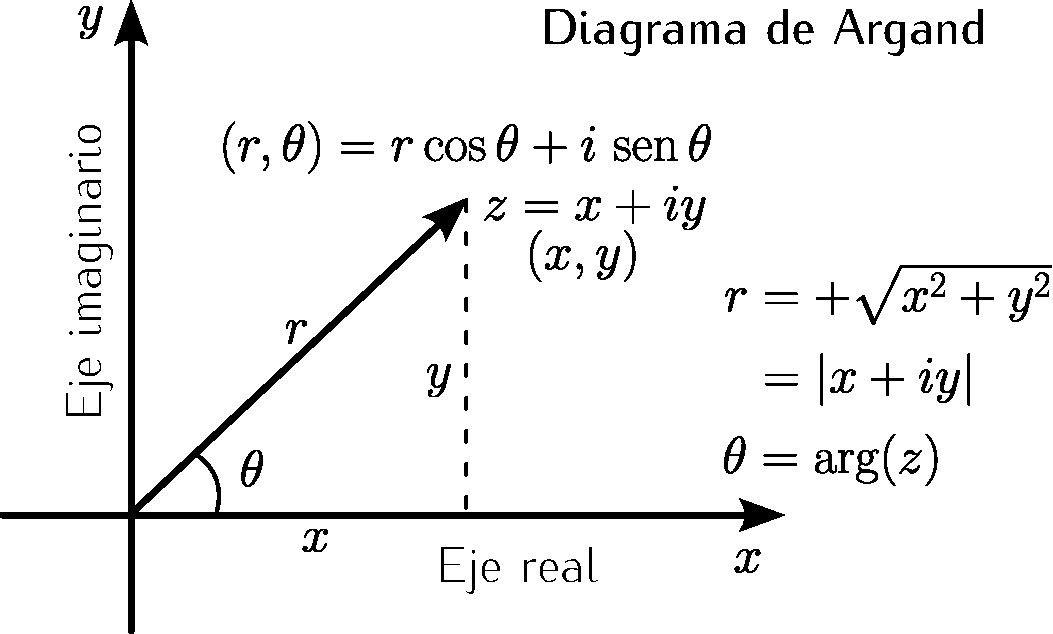
\includegraphics[width=1.0\textwidth]{figs/argand.pdf}
  \end{center}
\end{columns}
\end{frame}

\begin{frame}
 \begin{columns}[t]
  \cw{0.25}
  Estructura adicional de $\mathbb{C}$:
  \begin{align*}
   (4)&\; (a + ib)(c + id) = \\
   &= (ac - bd) + i (bc + ad)
  \end{align*}
  Caso especial:
  \begin{align*}
   (a + ib)(a - ib) &= a^2 + b^2 \geq 0 \\
   &= |a + i b|^2
  \end{align*}
  \textbf{Definición:} el complejo conjugado de $z = x + y i$ es
  \[ \bar{z} = x - y i \]
    \begin{center}
    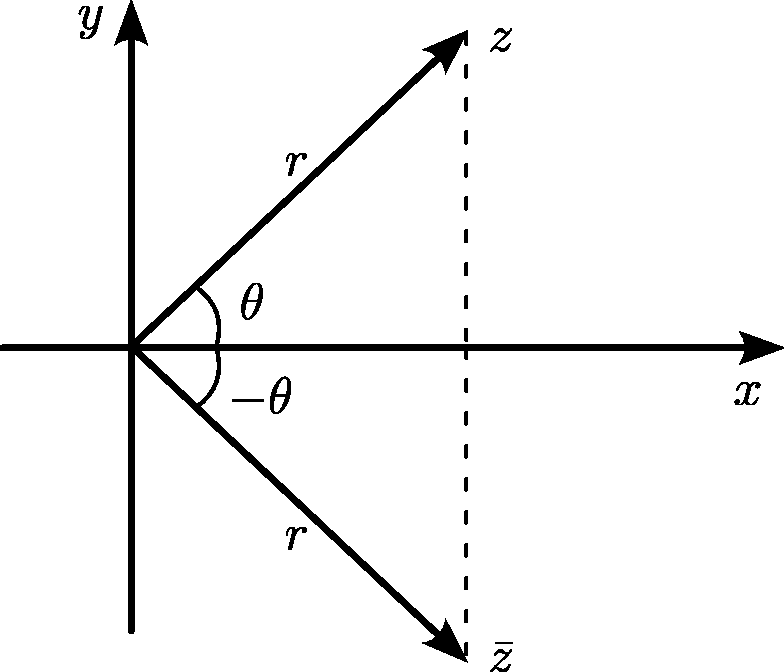
\includegraphics[scale=0.25]{figs/conjugado.pdf}
    \end{center}
  
  \cw{0.25}
  \begin{align*}
   \frac{c + di}{a + bi} &= \frac{c + di}{a + bi} \frac{a - bi}{a - bi} \\
   &= \frac{(ac + bd) + (ad - bc)i}{a^2 + b^2}
  \end{align*}
  \begin{align*}
   \frac{3 + 2 i}{4 + i} &= \frac{(3 + 2i)(4 - i)}{(4 + i)(4 - i)} \\
   &= \frac{14 + 5 i}{17} \\
   &= \frac{14}{17} + \frac{5}{17}i
  \end{align*}
  
  \[ \therefore \frac{\text{complejo}}{\text{complejo}} = \text{complejo} \]
  (excepto para división por cero).

  \cw{0.4}
  Producto en coordenadas polares:
  \begin{multline*}
   (r_1, \theta_1)(r_2, \theta_2) = (r_1 \cos \theta_1 + i r_1 \sen \theta_1) \\
   (r_2 \cos \theta_2 + i r_2 \sen \theta_2)= \\
   r_1 r_2 (\cos \theta_1 \cos \theta_2 - \sen \theta_1 \sen \theta_2) + \\
   i r_1 r_2 (\sen \theta_1 \cos \theta_2 + \sen \theta_2 \cos \theta_1) = \\
   r_1 r_2 \cos(\theta_1 + \theta_2) + i r_1 r_2 \sen(\theta_1 + \theta_2) = \\
   \boxed{ (r_1 r_2, \theta_1 + \theta_2) } \qquad
  \end{multline*}
  Por inducción:
  \begin{multline*}
   (r_1, \theta_1) \cdots (r_n, \theta_n) = \\
   (r_1 \cdots r_n, \theta_1 + \cdots + \theta_n)
  \end{multline*}
  Caso especial:
  \[ (r, \theta)^n = (r^n, n \theta) \]
   \[ \therefore r = 1 \rightarrow (1, \theta)^n = (1, n \theta) \]
 \end{columns}
\end{frame}


\begin{frame}
 \begin{columns}[t]
  \cx
  Teorema de De Moivre:
  \[  (\cos \theta + i \sen \theta)^n = \cos n \theta + i \sen n \theta \]
  
  Ejemplo:
  \begin{multline*}
   (\cos \theta + i \sen \theta)^2 = \cos 2 \theta + i \sen 2 \theta \\
 (\cos^2 \theta - \sen^2 \theta) + i 2 \sen \theta \cos \theta \\
 \end{multline*}

 \begin{align*}
 \therefore \;\sen 2 \theta &= 2 \sen \theta \cos \theta \\
 \cos 2 \theta & = \cos^2 \theta - \sen^2 \theta
 \end{align*}

 
  \cx
 Raíces: encontrar 
\begin{equation*}
\sqrt[6]{i} = x + i y \rightarrow i = (x + i y)^6 = 0 + 1 i
\end{equation*}
 
  \begin{align*}
   \therefore \; & x^6 + 15 x^4 (iy)^2 + 15 x^2 (iy)^4 + (iy)^6  \onslide<2->{\textcolor{red}{ = 0}} \\ 
   & + 6 x^5 (iy) + 20 x^3 (iy)^3 + 6x (iy)^5 \onslide<2->{\textcolor{red}{ = 1}}
  \end{align*}
  Sistema complicado a resolver:
  \begin{equation*}
   \begin{cases}
    x^6 + 15 x^4 (iy)^2 + 15 x^2 (iy)^4 + (iy)^6 = 0 \\
    6 x^5 (iy) + 20 x^3 (iy)^3 + 6x (iy)^5 = 1
   \end{cases}
  \end{equation*}
   \end{columns}
\end{frame}

\begin{frame}
 \begin{columns}[t]
  \cx
  En coordenadas polares:
  \begin{align*}
   &i = (1, \pi/2) \therefore \; \sqrt[6]{i} = (r, \theta) \\
   & \rightarrow  i = (r, \theta)^6 = (r^6, 6 \theta) \\
   & \therefore r = 1, \quad 6 \theta = \frac{\pi}{2} \textcolor{red}{+ 2 \pi k} = \frac{1 + 4 k}{2} \pi
  \end{align*}
  
   \begin{align*}
   r =& 1, \\
   \theta = &\frac{\pi}{12}, \frac{5 \pi}{12}, \frac{ 9 \pi}{12}, \frac{13 \pi}{12}, \frac{17 \pi}{12}, \frac{21 \pi}{12}, \\
   &\frac{25 \pi}{12}, \cdots
  \end{align*}
  
  \begin{align*}
   \left( 1, \dfrac{3 \pi}{4} \right) &= \cos \dfrac{3 \pi}{4} + i \sen \dfrac{3 \pi}{4} \\
   &= \frac{1}{\sqrt{2}} (-1 + i)
  \end{align*}


  \cx
  \begin{center}
    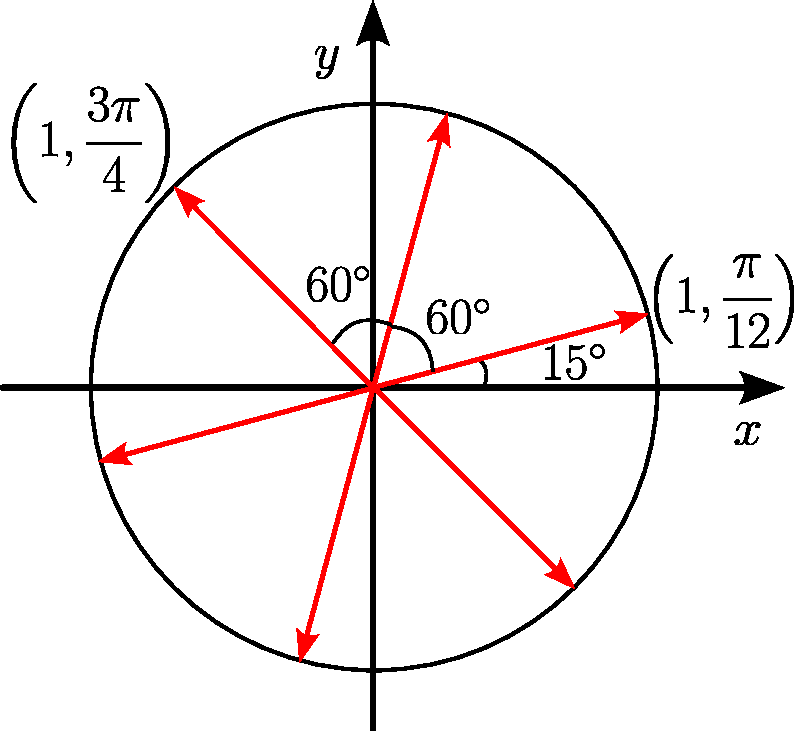
\includegraphics[scale=0.35]{figs/raices.pdf}
  \end{center}
  
  \begin{block}{Sistema de números complejos:}
   Los números complejos son \textbf{cerrados}
   respecto de la radicación.
  \end{block} 
 \end{columns}
\end{frame}

\begin{frame}[standout]
 Pausa para resolver problemas: 1 -- 8.
\end{frame}


%%%%%%%%%%%%%%%%%%%%%%%%%%%%%%%%%%%%%%%%%%%%%%%%%%%%%%%%%%%%%%%%%%%%%%%%%
% Fuente de esta presentación:
%       https://youtu.be/rVvGqWyQB_0
% del curso:
%  Calculus Revisited: Complex Variables, Differential Equations, and Linear Algebra
%   https://ocw.mit.edu/courses/res-18-008-calculus-revisited-complex-variables-differential-equations-and-linear-algebra-fall-2011/
%%%%%%%%%%%%%%%%%%%%%%%%%%%%%%%%%%%%%%%%%%%%%%%%%%%%%%%%%%%%%%%%%%%%%%%%%



\begin{frame}{Funciones de variable compleja}
 \begin{columns}[c]
  \cw{0.4}
  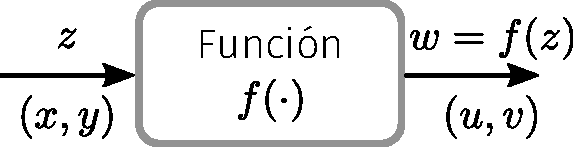
\includegraphics[width=0.9\textwidth]{figs/fig-01} \pause
  \cw{0.6}
  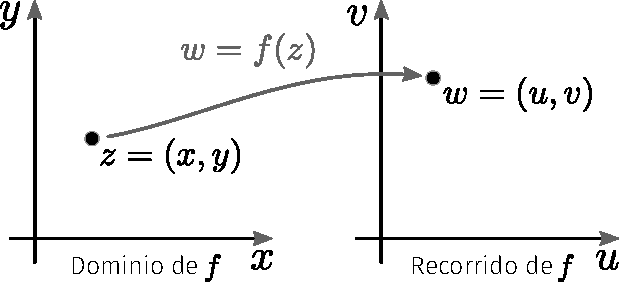
\includegraphics[width=0.9\textwidth]{figs/fig-02}
 \end{columns} \pause
 
 \begin{columns}[c]
  \cw{0.6}
 \begin{exampleblock}{Ejemplo:}
  \begin{align*}
   f(z) &= z^2 = (x + iy)^2 \\
        &= x^2 + 2 x i y + i^2 y^2 = x^2 - y^2 + 2 i xy \\
   \therefore f(x, y) &= (x^2 - y^2, 2xy)
  \end{align*}
 \end{exampleblock} \pause
  \cw{0.3}
  $\therefore f(z) = z^2$ es equivalente al \alert{sistema real}: 
  \vspace{1em}
  \[
  \begin{cases*}
   u = x^2 + y^2 \\
   v = 2xy
  \end{cases*}
  \]
 \end{columns}
\end{frame}


\begin{frame}{Límites}
 $\mathbb{C}$: números complejos \\
 $f: \mathbb{C} \mapsto \mathbb{C}, a \in \mathbb{C}$
 
 \begin{columns}[c]
  \cw{0.5}
 \begin{alertblock}{Definición:}
  \[ \lim_{z \rightarrow a} f(z) = L \]
  
  dado $\epsilon >0$ existe $\delta > 0$ tal que
  \[ 0 < |z - a| < \delta \rightarrowtail |f(z) - L| < \epsilon \]
 \end{alertblock} \pause
  \cw{0.5}
  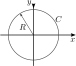
\includegraphics[width=0.9\textwidth]{figs/fig-03}
 \end{columns} \pause
 
 \noindent Los teoremas usuales sobre límites \alert{son válidos}. En particular: \vspace{0.5em}
 
 \begin{columns}[t]
  \cw{0.3}
  Si
  \begin{align*}
   f(z) &= u(x, y) + i v(x, y) \\
   L &= L_1 + i L_2 \\
   a &= a_1 + i a_2
  \end{align*}
  \cw{0.6}
  Entonces:
  \[ \lim_{z \rightarrow a} f(z) = L \longleftrightarrow
  \begin{cases}
    \lim_{(x,y) \rightarrow (a_1, a_2)} u(x, y) = L_1  \\
    \lim_{(x,y) \rightarrow (a_1, a_2)} v(x, y) = L_2
  \end{cases}
  \]
 \end{columns}
\end{frame}


\begin{frame}{Derivada}
 \begin{columns}
  \cw{0.5}
  \begin{alertblock}{Definición:}
   \[ f'(z_0) = \lim_{\Delta z \rightarrow 0} \left[ \frac{f(z_0 + \Delta z) - f(z_0)}{\Delta z} \right] ¨ \]
  \end{alertblock} \pause
  \vspace{2em}
  
  Si $w = f(z) = u(x, y) + i v(x, y)$:
  \begin{align*}
   f'(z_0) &= \frac{dw}{dz} = \lim_{\Delta z \rightarrow 0} \frac{\Delta w}{\Delta z} \\
           &= \lim_{\Delta z \rightarrow 0} \left[ \frac{\Delta u + i \Delta v}{\Delta x + i \Delta y} \right]
  \end{align*} \pause
  
  \cw{0.5}
  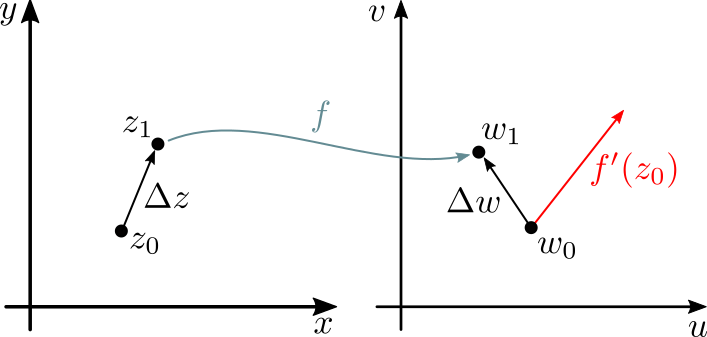
\includegraphics[width=0.9\textwidth]{figs/fig-04b.png}
 \end{columns}
\end{frame}

\begin{frame}{Derivada: casos especiales}
 \begin{columns}[t]
  \cw{0.4}
  \textbf{Caso 1:} $\Delta y \equiv 0$.
  \begin{align*}
   \therefore f'(z_0) &= \lim_{\Delta x \rightarrow 0} \left[ \frac{\Delta u}{\Delta x} + i \frac{\Delta v}{\Delta x} \right] \\
   &= \frac{\partial u}{\partial x} + i \frac{\partial v}{\partial x} \biggr\rvert_{z_0 = (x_0, y_0)}
  \end{align*} \pause

  \cw{0.6}
  \textbf{Caso 2:} $\Delta x \equiv 0$.
  \begin{align*}
   \therefore f'(z_0) &= \lim_{\Delta y \rightarrow 0} \left[ \frac{\Delta u}{i \Delta y} +  \frac{\Delta v}{\Delta y} \right] = \frac{\partial v}{\partial y} + \frac{1}{i} \frac{\partial u}{\partial y} \biggr\rvert_{z_0 = (x_0, y_0)} \\
   &= \frac{\partial v}{\partial y} - i \frac{\partial u}{\partial y} \biggr\rvert_{z_0 = (x_0, y_0)}
  \end{align*} \pause
 \end{columns}
 \vspace{2em}
 
 \begin{block}{Ecuaciones de Cauchy-Riemann}
 \begin{center}
  Si $f = u + i v$ es diferenciable (\alert{analítica}), entonces:
  \begin{align*}
    u_x &= v_y \\
    u_y &= -v_x
  \end{align*}
  \end{center}
 \end{block}
\end{frame}

\begin{frame}{Derivada: ejemplo 1}
 \begin{columns}[t]
  \cw{0.4}
  Ecuaciones de Cauchy-Riemann:
  
  \begin{align*}
   f(z) &= z^2 = (x + i y)^2 \\
        &= (x^2 - y^2) + i (2xy)
  \end{align*}
  \[\left.{ \begin{array}{ll}
             u_x = 2 x, & v_x = 2 y \\
             u_y = -2y, & v_y = 2 x 
            \end{array}}  \right\}
            \Rightarrow \begin{array}{l}
               u_x = v_y \\
               u_y = -v_x
              \end{array}
 \]
 \pause
 
  \cw{0.6}
  Derivada por definición:
  
  \begin{align*}
   \frac{f(z_0 + \Delta z) - f(z_0)}{\Delta z} &= \frac{(z_0 + \Delta z)^2 - z_0^2}{\Delta z} \\
   &= \frac{2 z_0 \Delta z + \Delta z^2}{\Delta z} \quad (\Delta z \neq 0)\\
   &= 2 z_0 + \Delta z \\
   \therefore \hspace{1em} \Aboxed{ f'(z_0) &= 2 z_0 }
  \end{align*}
 \end{columns}
\end{frame}

\begin{frame}{Derivada: ejemplo 2}
 \begin{columns}[c]
  \cw{0.5}
  \[
  \begin{array}{c}
   f(z) = \bar{z} = x - i y \\
   u = x, \; v = -y \Rightarrow u_x \neq v_y 
   \end{array} \pause
   \] \vspace{1em}
  \begin{align*}
   \frac{\Delta w}{\Delta z} &= \frac{\Delta x - i \Delta y}{\Delta x + i \Delta y} \\
   &= \frac{1 - i \frac{\Delta y}{\Delta x}}{1 + i \frac{\Delta y}{\Delta x}} \rightarrow \frac{1 - \frac{dy}{dx}}{1 + i \frac{dy}{dx}}
  \end{align*} \pause

  \cw{0.5}
  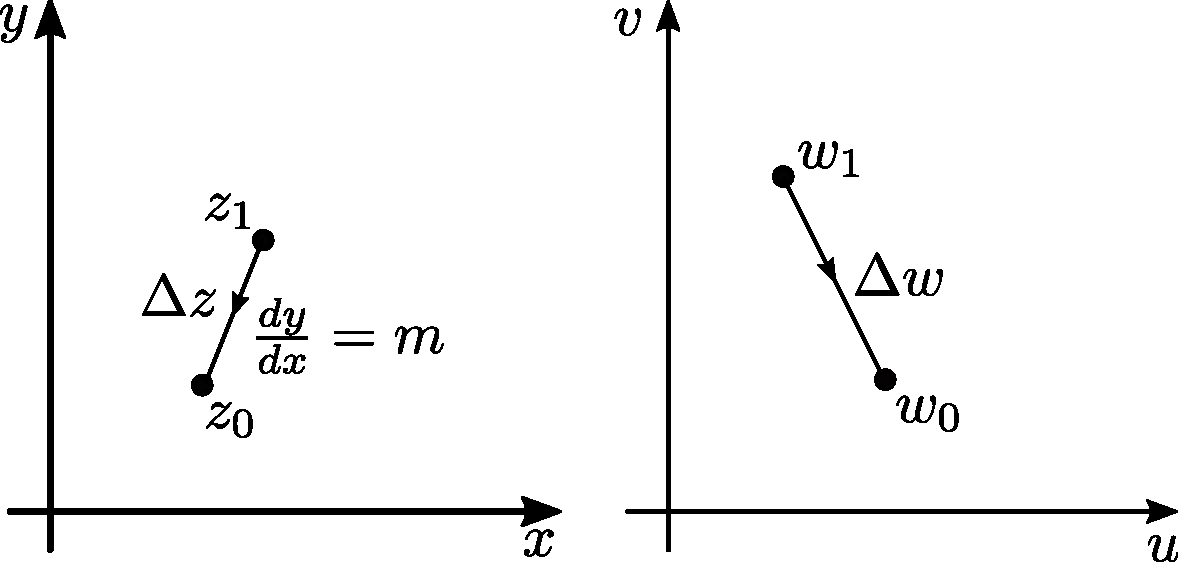
\includegraphics[width=0.9\textwidth]{figs/fig-05}
  
  \[ \frac{\Delta w}{\Delta z} = \frac{1 - im}{1 + im} = g(m) \]
 \end{columns}
\end{frame}

\begin{frame}{Aplicación: ecuación de Laplace y ejemplo}
$u(x, y)$ satisface la ecuación de Laplace si: 
\[\boxed{ \frac{\partial^2 u}{\partial x^2} + \frac{\partial^2 u}{\partial y^2} = 0 } \] \pause
\vspace{1em}

\begin{columns}[t]
 \cx
 Si $u + i v$ es \textbf{analítica}:
 \begin{align*}
  u_x = v_y \; &\therefore \; u_{xx} = v_{yx} \\
  u_y = -v_x \; &\therefore \; u_{yy} = -v_{xy} \\
 \end{align*} \vspace{-3em}
 \begin{align*}
  \frac{\partial^2 u}{\partial x^2} + \frac{\partial^2 u}{\partial y^2} &= 0 \\
  \frac{\partial^2 v}{\partial x^2} + \frac{\partial^2 v}{\partial y^2} &= 0
 \end{align*} \pause

 \cx
 \begin{exampleblock}{Ejemplo:}
 \[ f(z) = z^2 \longrightarrow 
 \begin{cases}
  u = x^2 - y^2 \\
  v = 2 x y
 \end{cases}
\]

\[
\therefore \left. { \begin{array}{ll}
                   u_{xx} + u_{yy} &= 0 \\
                   v_{xx} + v_{yy} &= 0 
                  \end{array} }
            \right\}
\]
 \end{exampleblock}
\end{columns}
\end{frame}


\section*{Bibliografía}
\begin{frame}[allowframebreaks]{Lecturas recomendadas}
\begin{itemize}
 \item \fullcite{kreyszig2011}. Capítulo 13.
 \item \fullcite{spiegel2011}. Capítulos 1 y 2.
\end{itemize}

% \nocite{kreyszig2011}
% \nocite{spiegel2011}
% \nocite{vesely2012}
% \nocite{thornton2015}
% \printbibliography
\end{frame}


\end{document}

